% mnras_template.tex 
%
% LaTeX template for creating an MNRAS paper
%
% v3.0 released 14 May 2015
% (version numbers match those of mnras.cls)
%
% Copyright (C) Royal Astronomical Society 2015
% Authors:
% Keith T. Smith (Royal Astronomical Society)

% Change log
%
% v3.0 May 2015
%    Renamed to match the new package name
%    Version number matches mnras.cls
%    A few minor tweaks to wording
% v1.0 September 2013
%    Beta testing only - never publicly released
%    First version: a simple (ish) template for creating an MNRAS paper

%%%%%%%%%%%%%%%%%%%%%%%%%%%%%%%%%%%%%%%%%%%%%%%%%%
% Basic setup. Most papers should leave these options alone.
\documentclass[fleqn,usenatbib]{mnras}

% MNRAS is set in Times font. If you don't have this installed (most LaTeX
% installations will be fine) or prefer the old Computer Modern fonts, comment
% out the following line
%\usepackage{newtxtext,newtxmath}
% Depending on your LaTeX fonts installation, you might get better results with one of these:
\usepackage{mathptmx}
%\usepackage{txfonts}

% Use vector fonts, so it zooms properly in on-screen viewing software
% Don't change these lines unless you know what you are doing
\usepackage[T1]{fontenc}

% Allow "Thomas van Noord" and "Simon de Laguarde" and alike to be sorted by "N" and "L" etc. in the bibliography.
% Write the name in the bibliography as "\VAN{Noord}{Van}{van} Noord, Thomas"
\DeclareRobustCommand{\VAN}[3]{#2}
\let\VANthebibliography\thebibliography
\def\thebibliography{\DeclareRobustCommand{\VAN}[3]{##3}\VANthebibliography}


%%%%% AUTHORS - PLACE YOUR OWN PACKAGES HERE %%%%%

% Only include extra packages if you really need them. Common packages are:
\usepackage{graphicx}	% Including figure files
\usepackage{amsmath}	% Advanced maths commands
\usepackage{amssymb}	% Extra maths symbols


%%%%%%%%%%%%%%%%%%%%%%%%%%%%%%%%%%%%%%%%%%%%%%%%%%

%%%%% AUTHORS - PLACE YOUR OWN COMMANDS HERE %%%%%

% Please keep new commands to a minimum, and use \newcommand not \def to avoid
% overwriting existing commands. Example:
%\newcommand{\pcm}{\,cm$^{-2}$}	% per cm-squared

%%%%%%%%%%%%%%%%%%%%%%%%%%%%%%%%%%%%%%%%%%%%%%%%%%

%%%%%%%%%%%%%%%%%%% TITLE PAGE %%%%%%%%%%%%%%%%%%%

% Title of the paper, and the short title which is used in the headers.
% Keep the title short and informative.
\title[S-PLUS: Emission line objects]{S-PLUS: Emission line objects in the southern photometric local Universe survey}

% The list of authors, and the short list which is used in the headers.
% If you need two or more lines of authors, add an extra line using \newauthor
\author[Guti\'{e}rrez-Soto et al.]{
L. A. Guti\'{e}rrez-Soto,$^{1}$\thanks{E-mail: gsoto.angel@gmail.com}
Second  Author,$^{2}$
Third Author$^{2,3}$
and Fourth Author$^{3}$
\\
% List of institutions
$^{1}$Departamento de Astronomia, IAG, Universidade de S\~{o}a Paulo, Rua do Mata\~{o}, 1226, 05509-900, S\~{o}a Paulo, Brazil\\
$^{2}$Department, Institution, Street Address, City Postal Code, Country\\
$^{3}$Another Department, Different Institution, Street Address, City Postal Code, Country
}

% These dates will be filled out by the publisher
\date{Accepted XXX. Received YYY; in original form ZZZ}

% Enter the current year, for the copyright statements etc.
\pubyear{2021}

% Don't change these lines
\begin{document}
\label{firstpage}
\pagerange{\pageref{firstpage}--\pageref{lastpage}}
\maketitle

% Abstract of the paper
\begin{abstract}
The emission line objects represent...
\end{abstract}

% Select between one and six entries from the list of approved keywords.
% Don't make up new ones.
\begin{keywords}
keyword1 -- keyword2 -- keyword3
\end{keywords}

%%%%%%%%%%%%%%%%%%%%%%%%%%%%%%%%%%%%%%%%%%%%%%%%%%

%%%%%%%%%%%%%%%%% BODY OF PAPER %%%%%%%%%%%%%%%%%%

\section{Introduction}

Large-scale H{$\alpha$} imaging surveys have traditionally focused on ex-
tended emission-line sources,
% \texttt{mnras\_sample.tex} for a more complex example, and \texttt{mnras\_guide.tex}

% \citet{Fournier1901},
% \citep[e.g.][]{vanDijk1902}.
% \citet{deLaguarde1903, delaGuarde1904}.


\section{Observations}
\label{sec:obser}

The S-PLUS survey is a multi-band photometric survey...

\begin{figure}
	% To include a figure from a file named example.*
	% Allowable file formats are eps or ps if compiling using latex
	% or pdf, png, jpg if compiling using pdflatex
	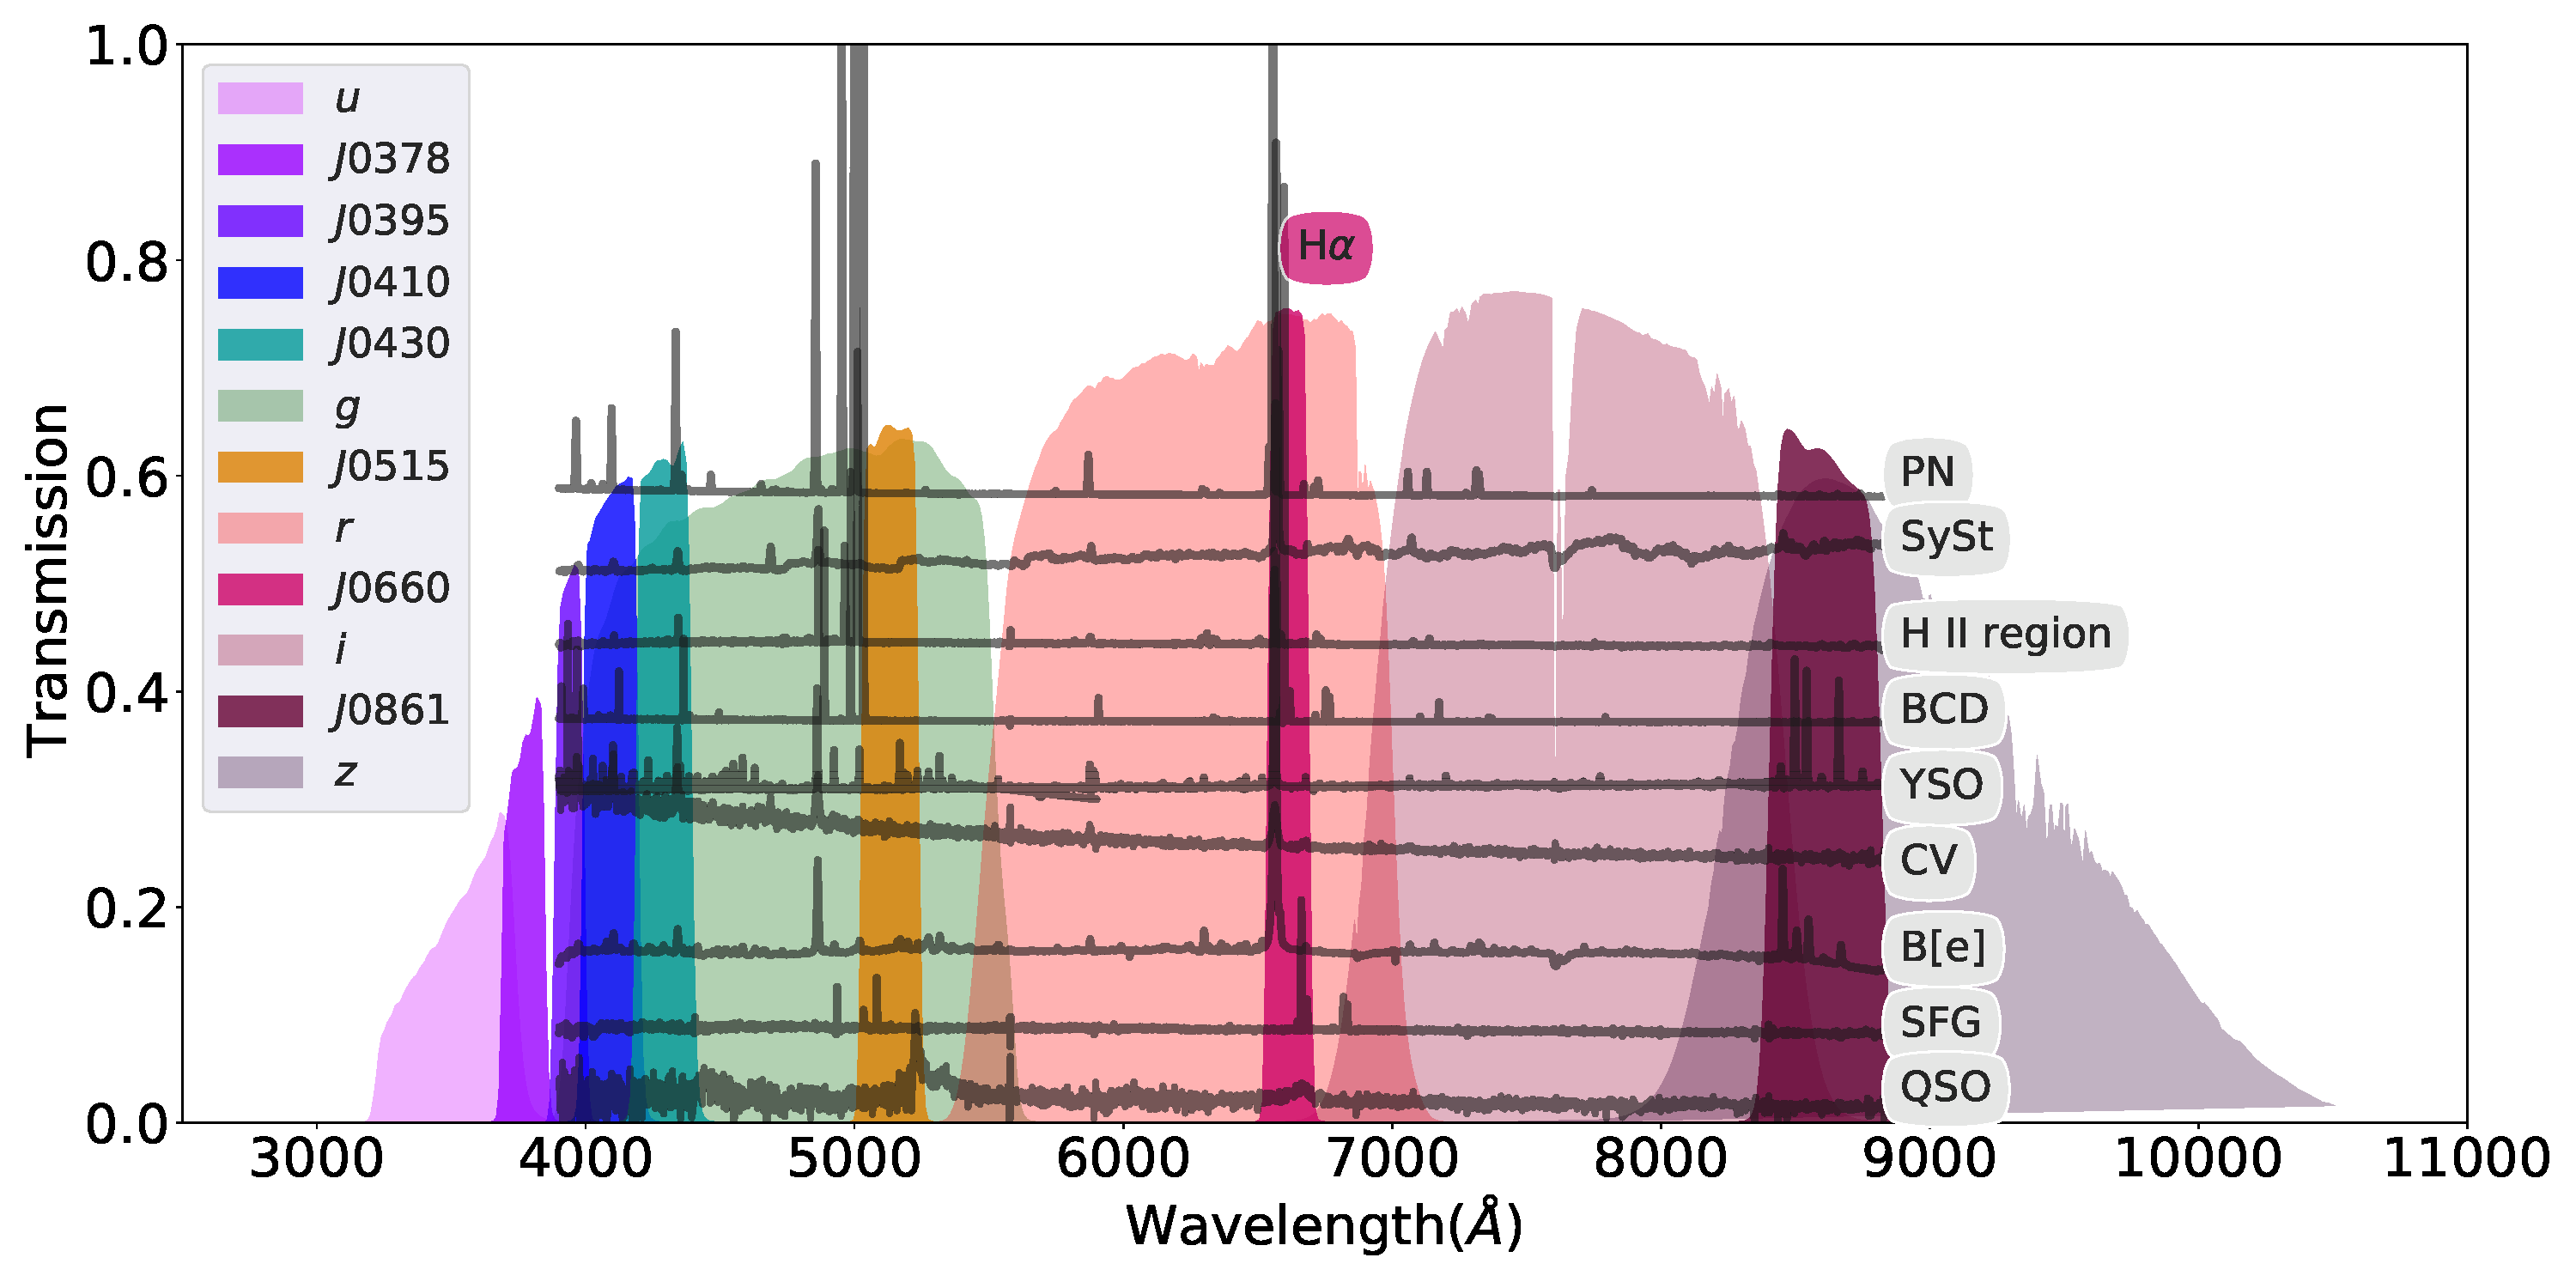
\includegraphics[width=\columnwidth]{Figs/splus-filter.pdf}
    \caption{Transmission curves...}
    \label{fig:curves}
\end{figure}


\section{Methodology}
\label{sec:meth}

\begin{figure*}
  \setlength\tabcolsep{0pt}
  \setkeys{Gin}{width=0.5\linewidth}
  \begin{tabular}{ll}
    (a) & (b) \\
    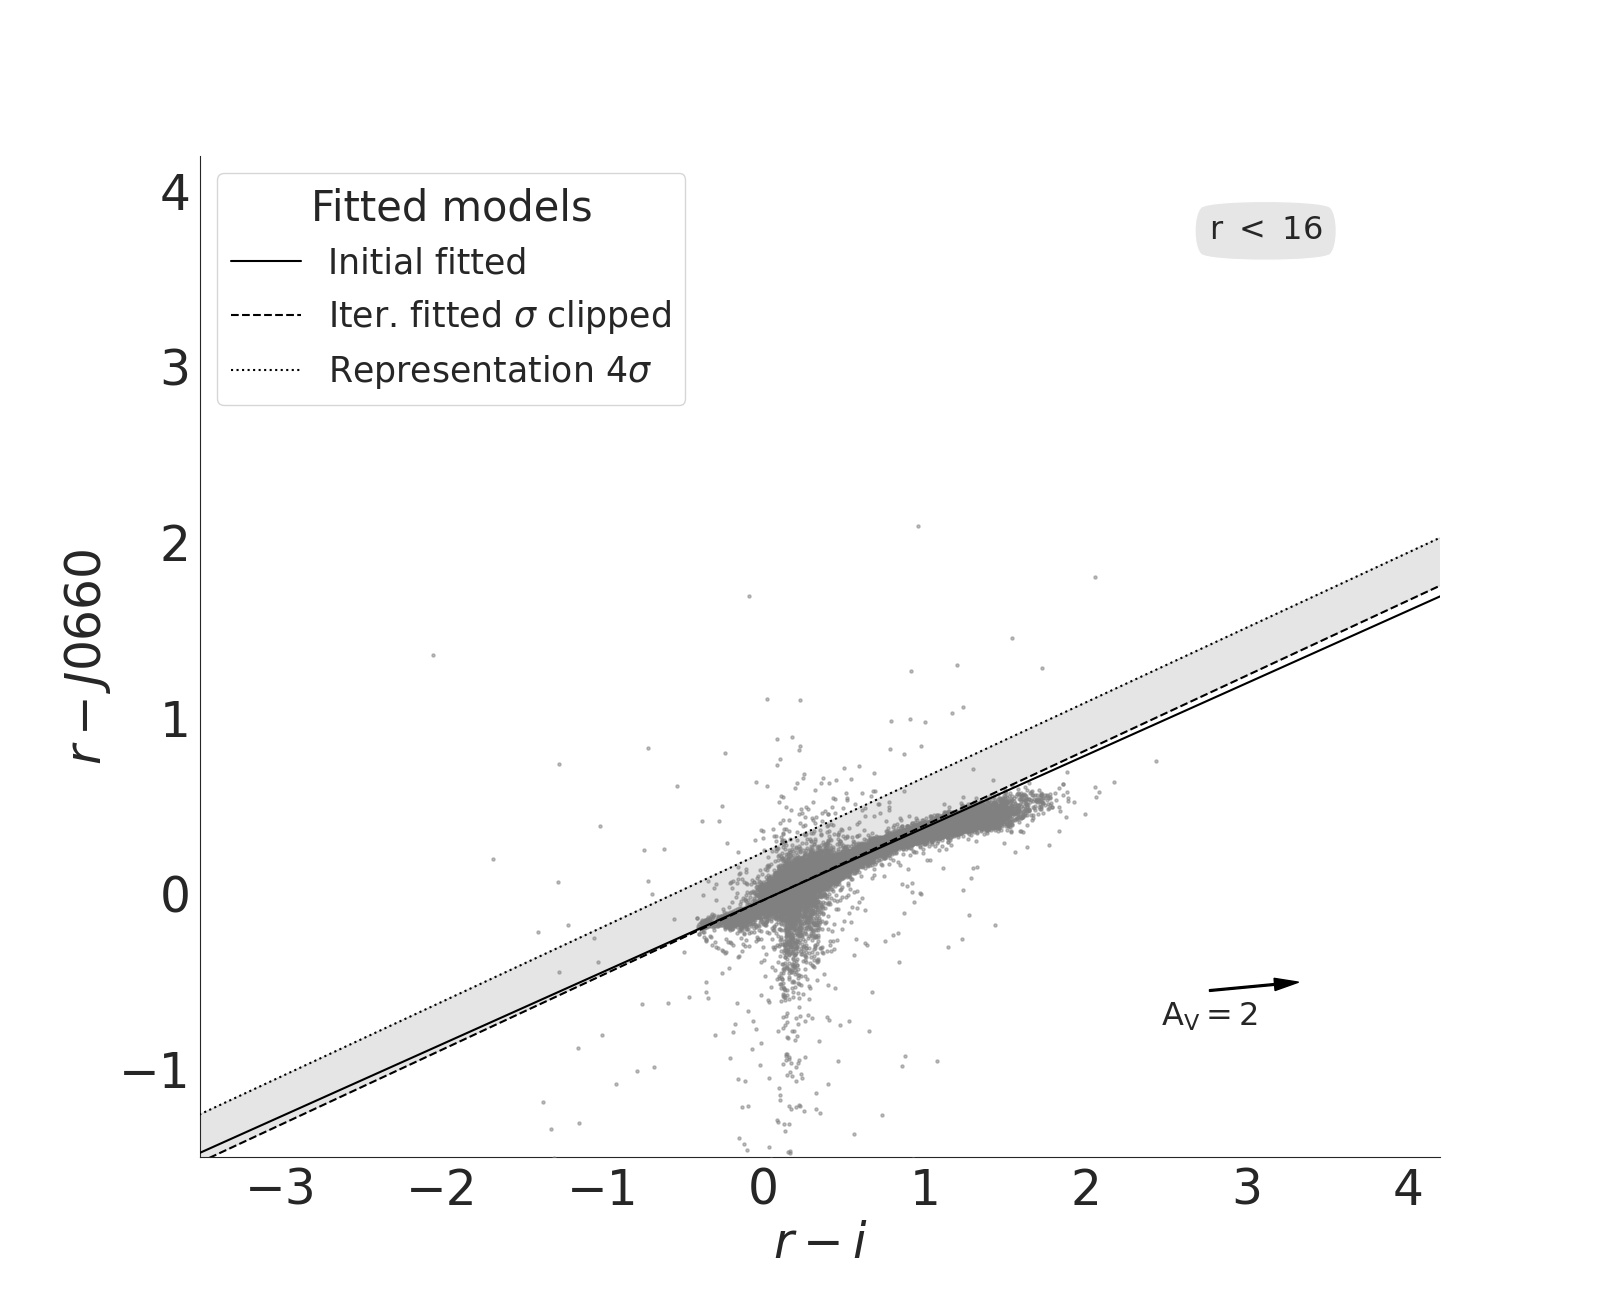
\includegraphics[trim=10 0 65 20, clip]{Figs/diagram-DR3-errorFlag0-3f-16r}
    & 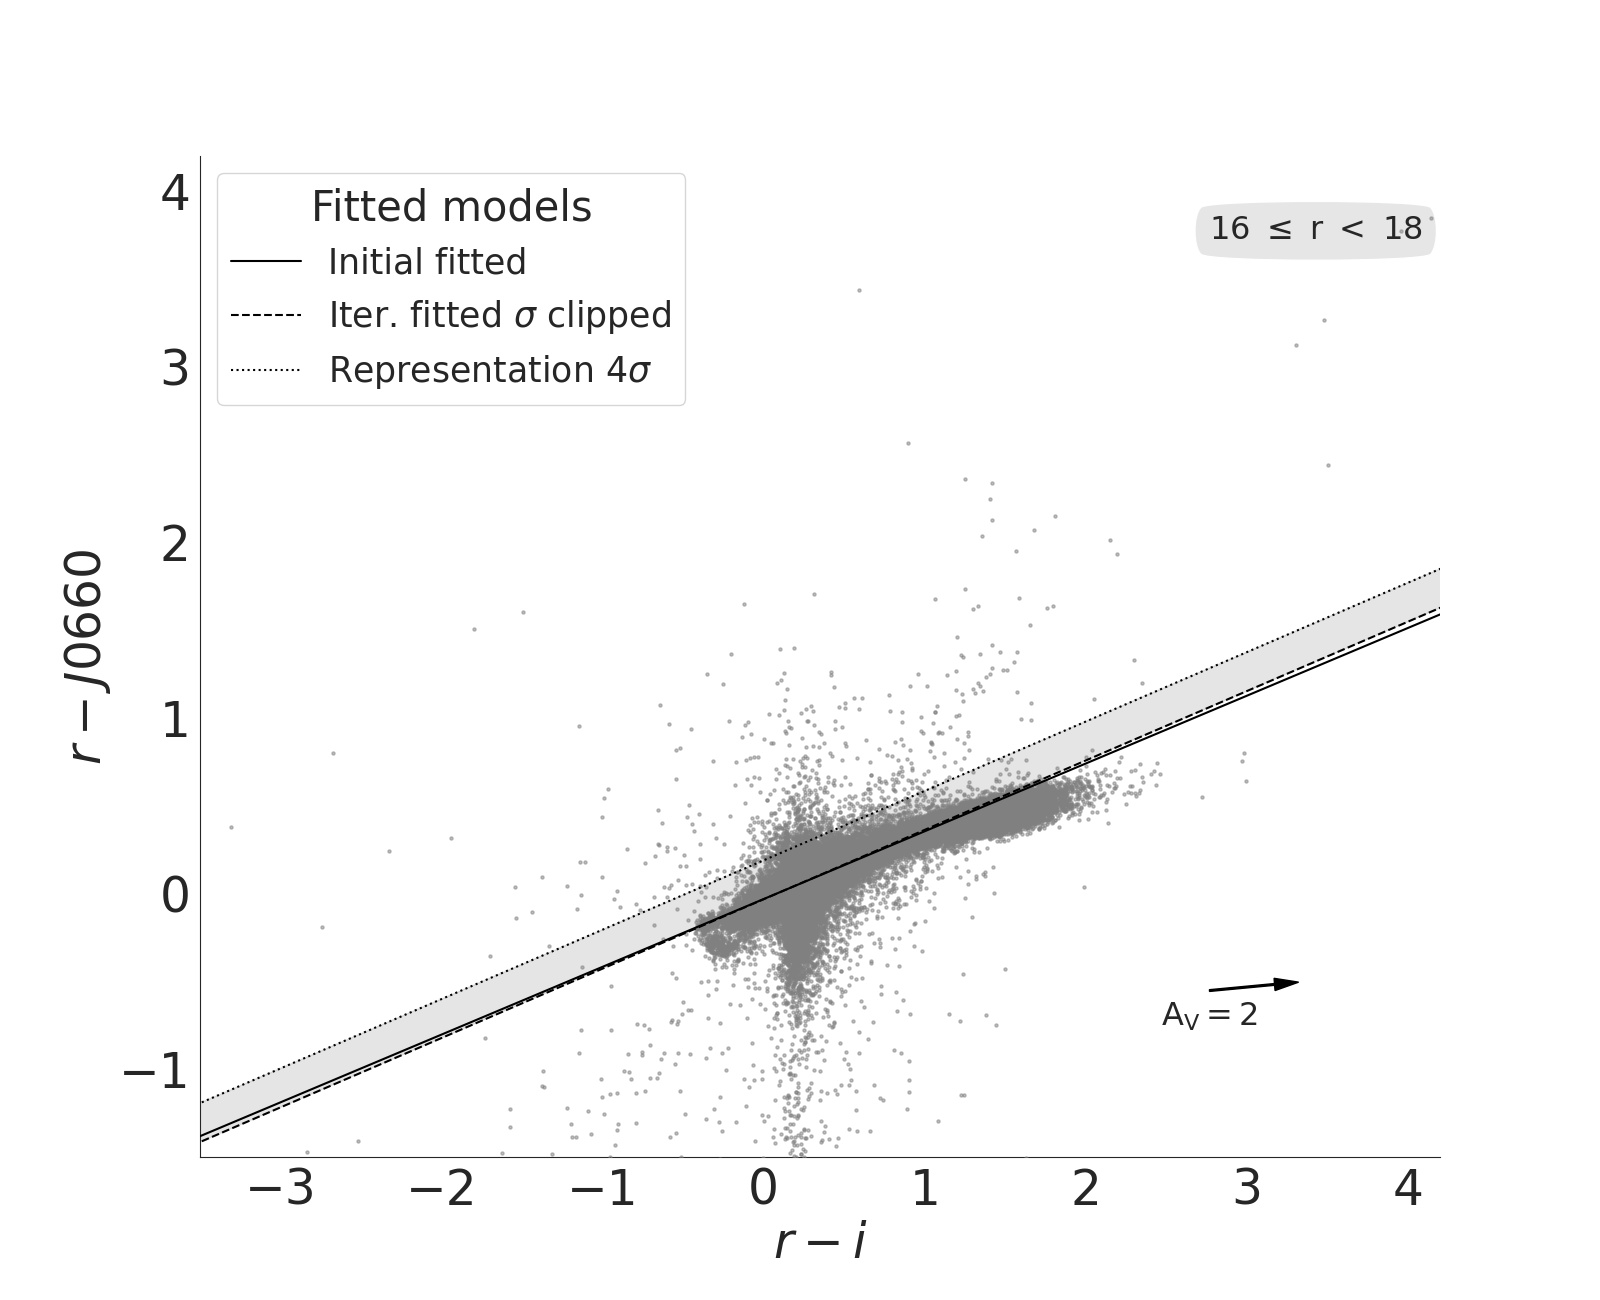
\includegraphics[trim=10 0 65 20, clip]{Figs/diagram-DR3-errorFlag0-3f-16r18}\\
    (c) & (d) \\
    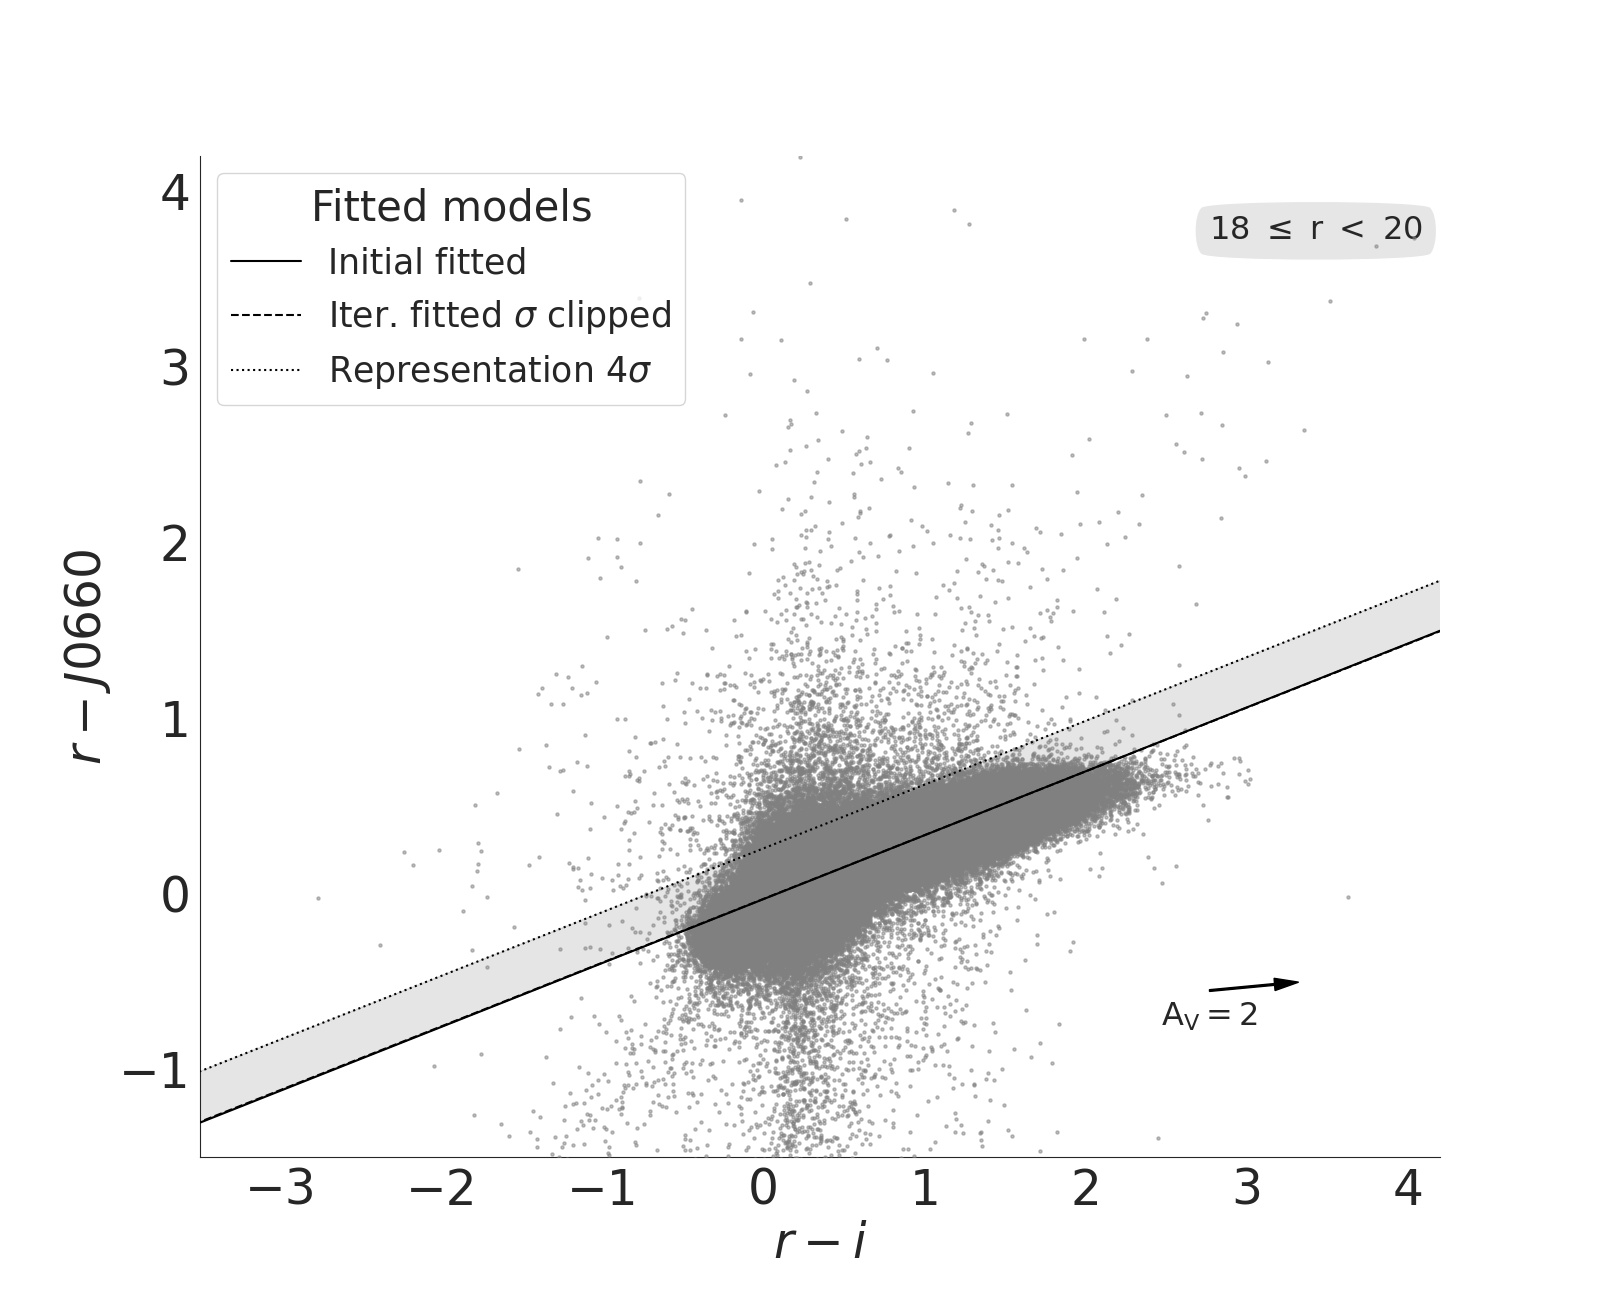
\includegraphics[trim=10 0 65 20, clip]{Figs/diagram-DR3-errorFlag0-3f-18r20}
    & 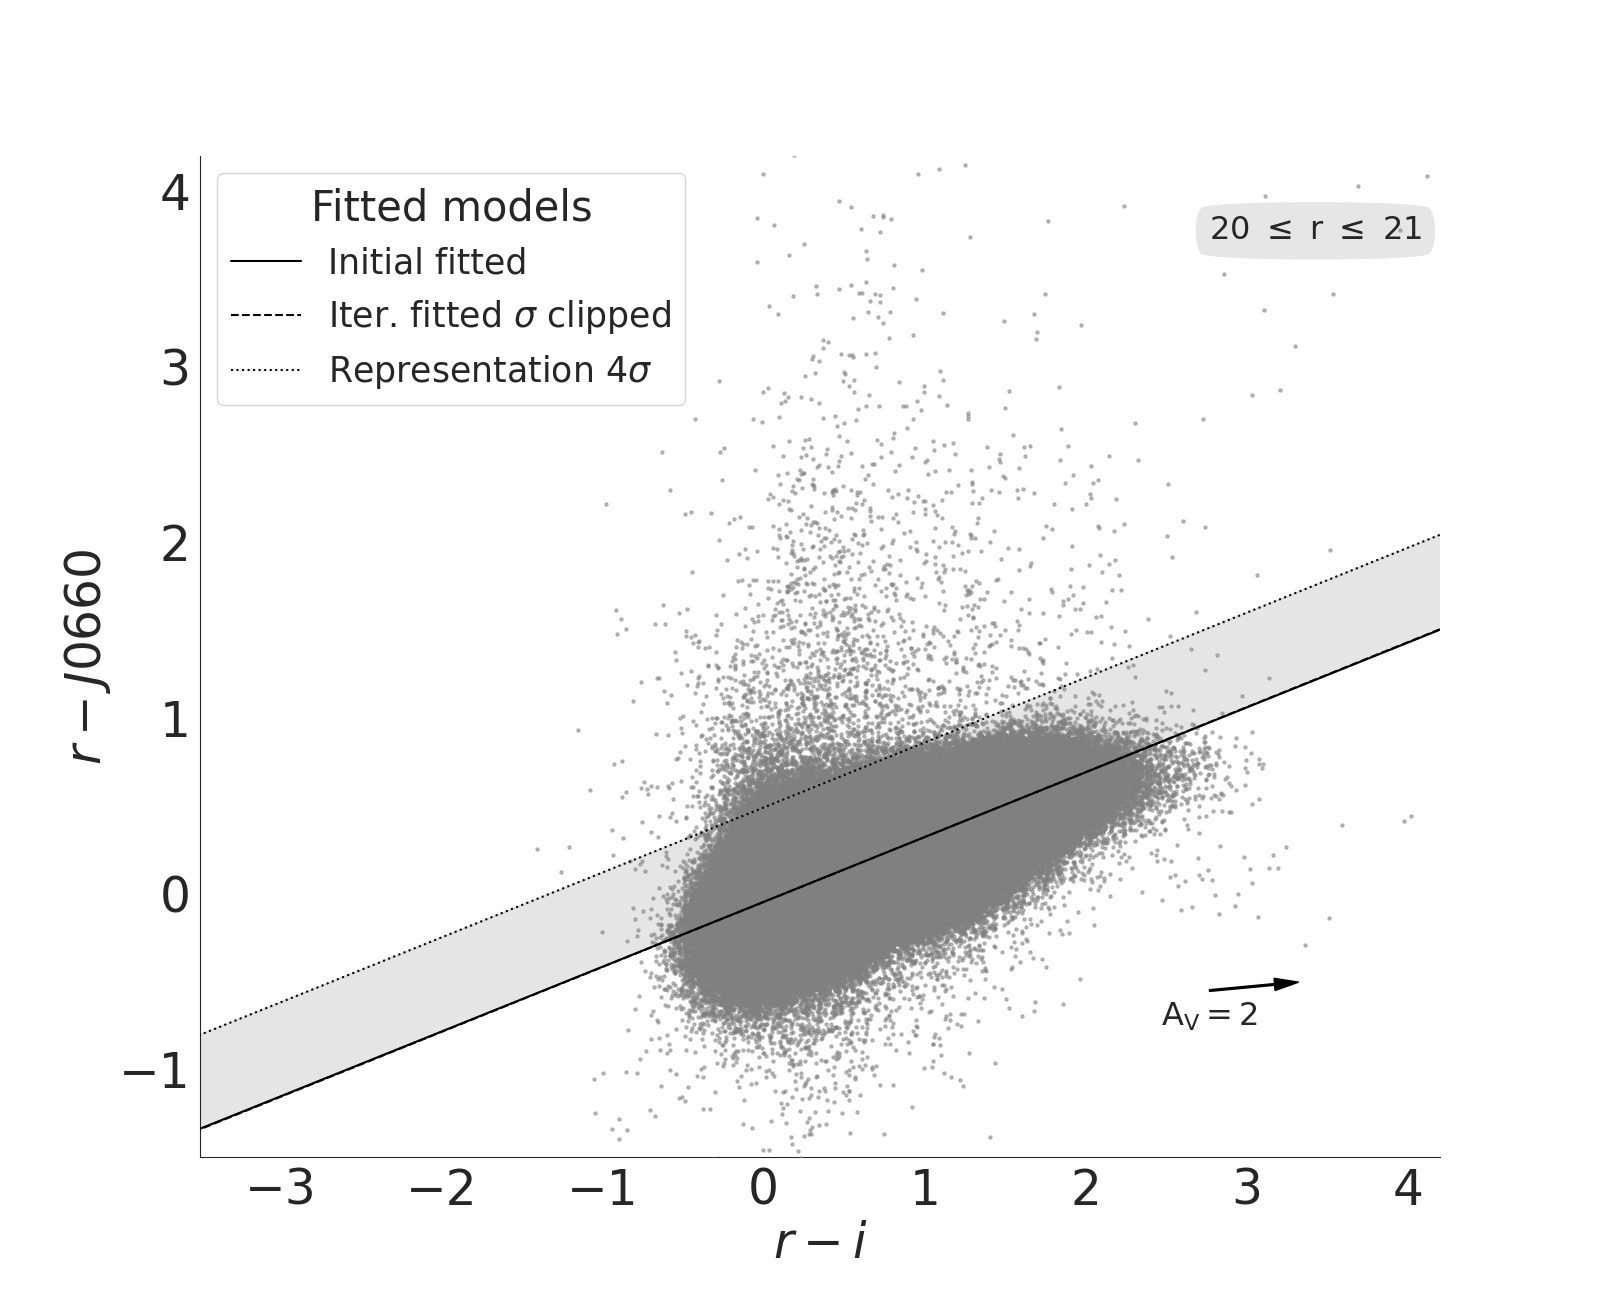
\includegraphics[trim=10 0 65 20, clip]{Figs/diagram-DR3-errorFlag0-3f-20r21}\\
  \end{tabular}
  \caption{Color-color diagrams with all objects...}
  \label{fig:color-diagram}
\end{figure*}


%It is frequently split into subsections, such as Section~\ref{sec:maths} below.

\subsection{Maths}
\label{sec:maths} % used for referring to this section from elsewhere

 %% e.g. $2\times3=6$
%% or $v=220$\,km\,s$^{-1}$, but more complicated expressions should be entered


\begin{equation}

    x=\frac{-b\pm\sqrt{b^2-4ac}}{2a}.
	\label{eq:quadratic}
\end{equation}

%Refer back to them as e.g. equation~(\ref{eq:quadratic}).

\subsection{Figures and tables}

\section{Results}
\label{sec:results}

\begin{figure}
	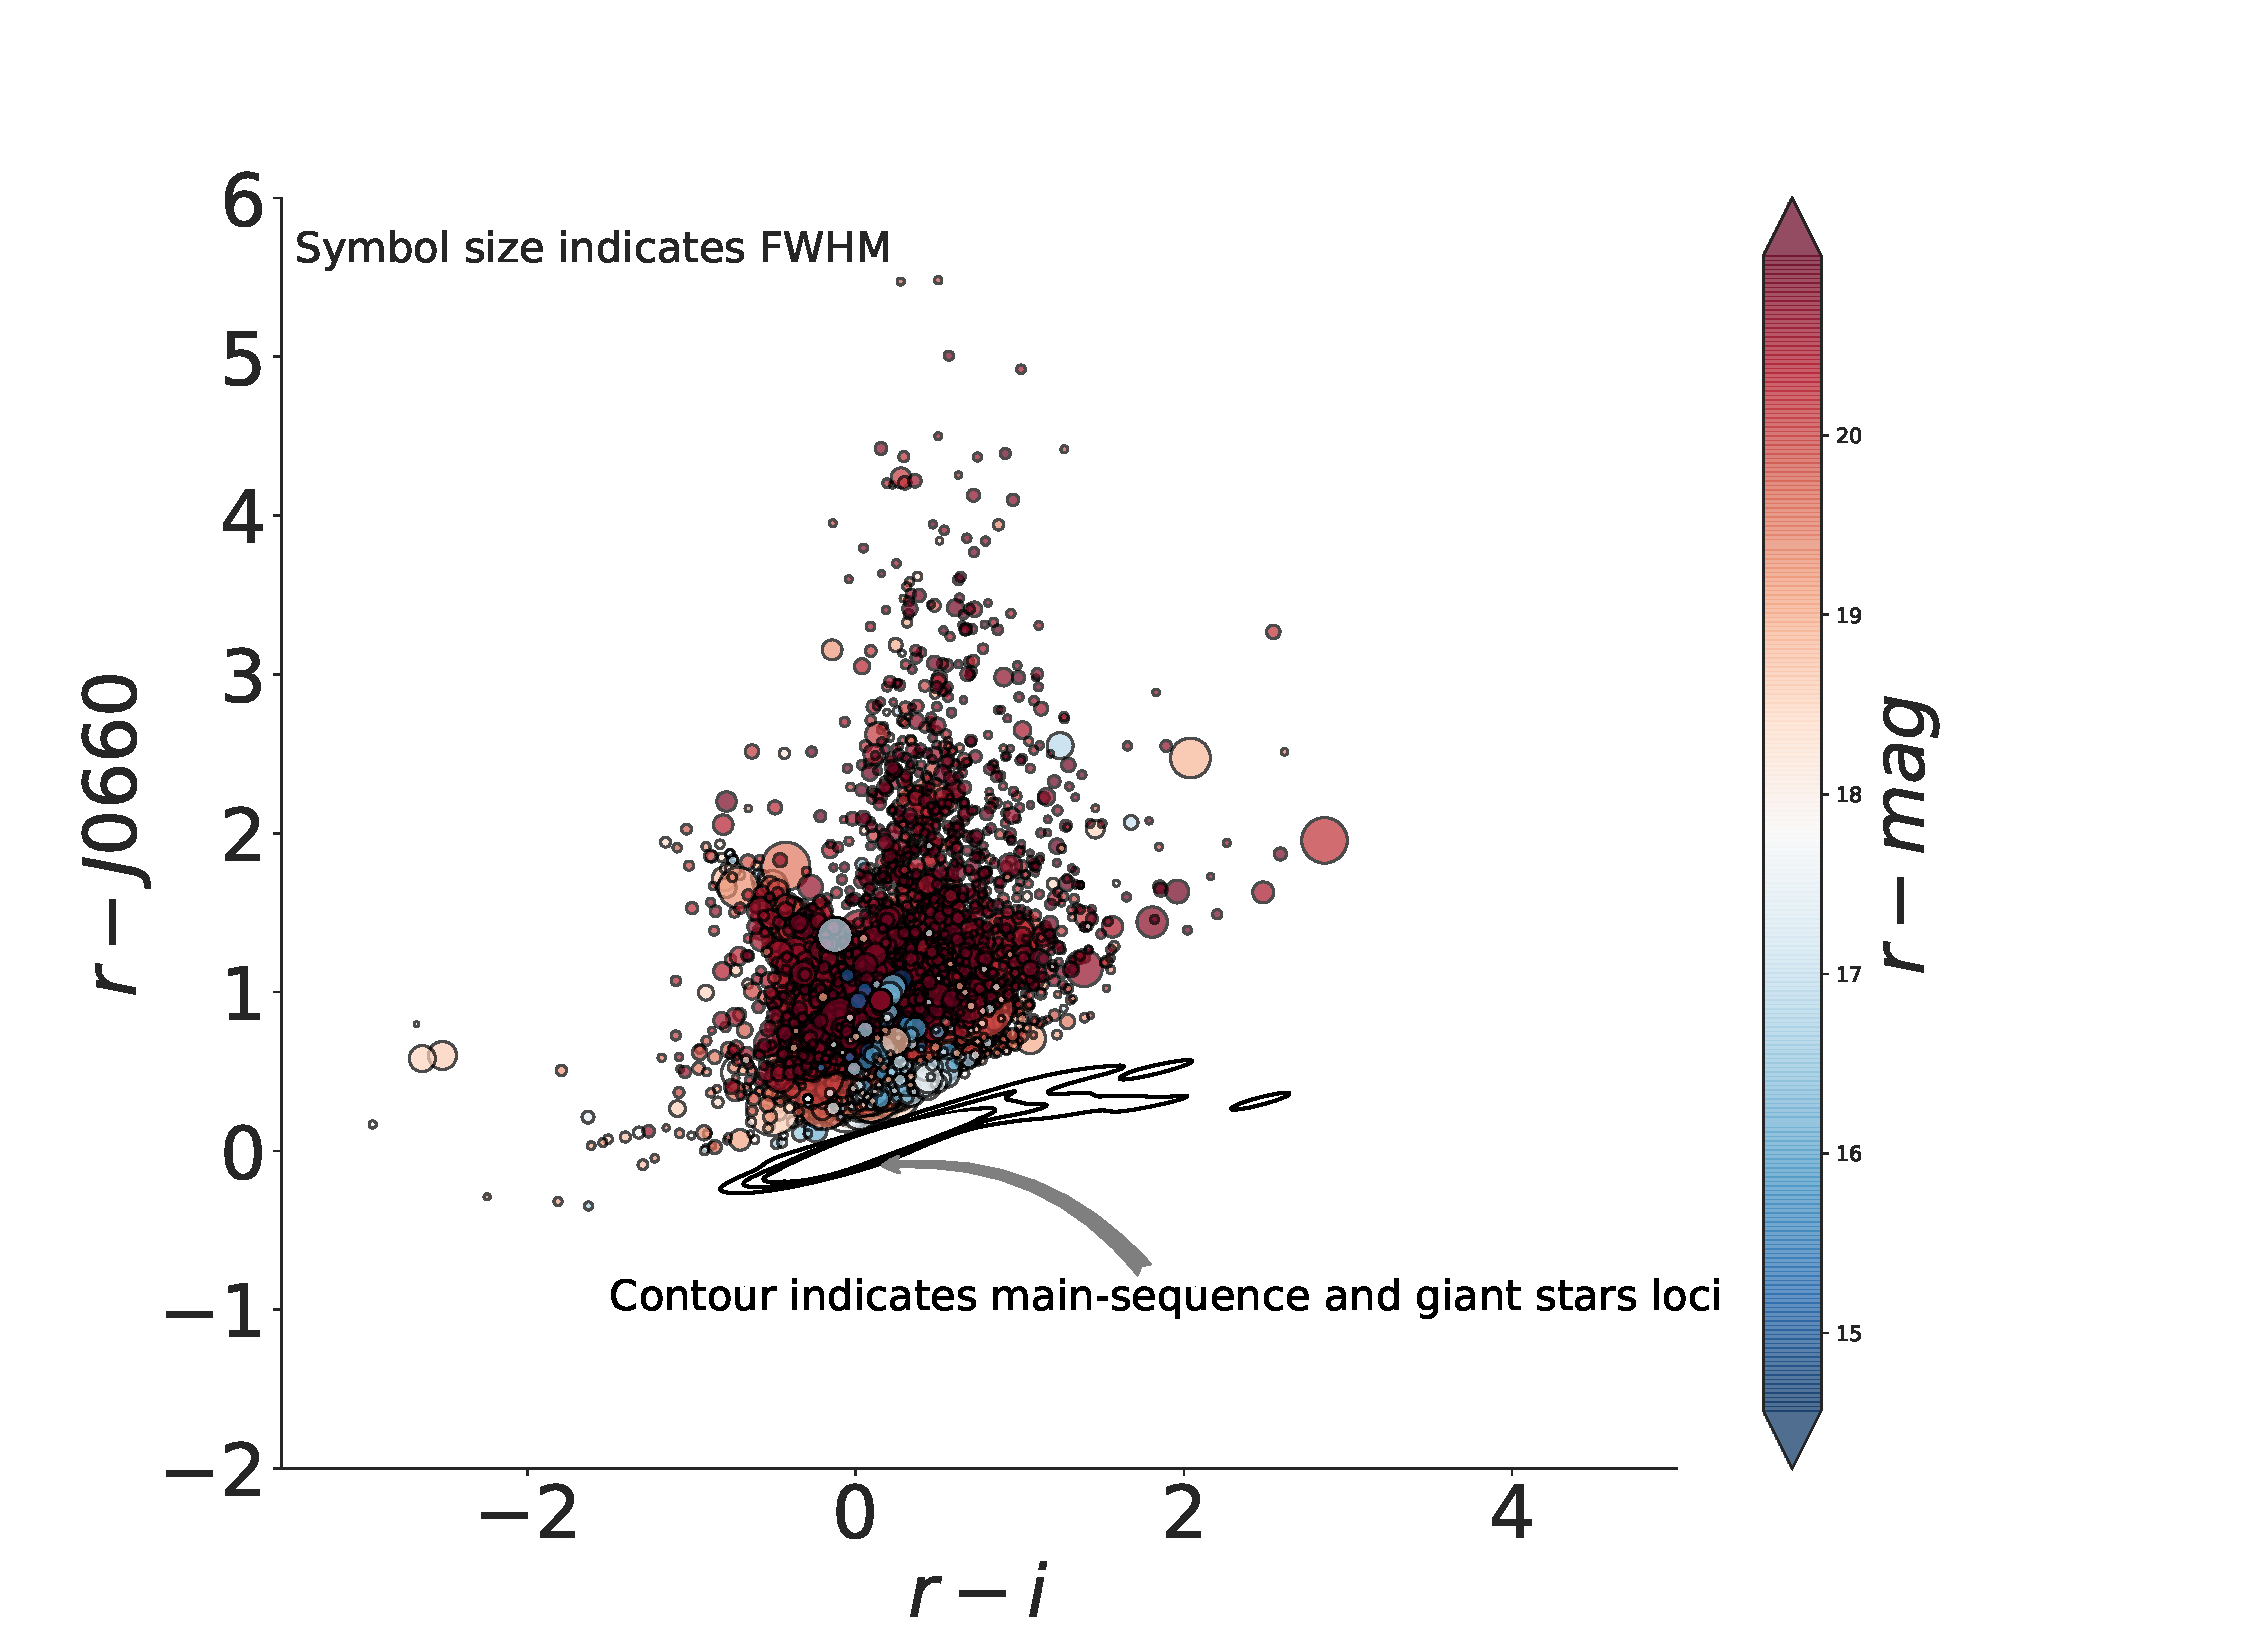
\includegraphics[width=\columnwidth]{Figs/final-emitters.pdf}
    \caption{Emission lines selected...}
    \label{fig:emiss}
\end{figure}

\begin{figure}
	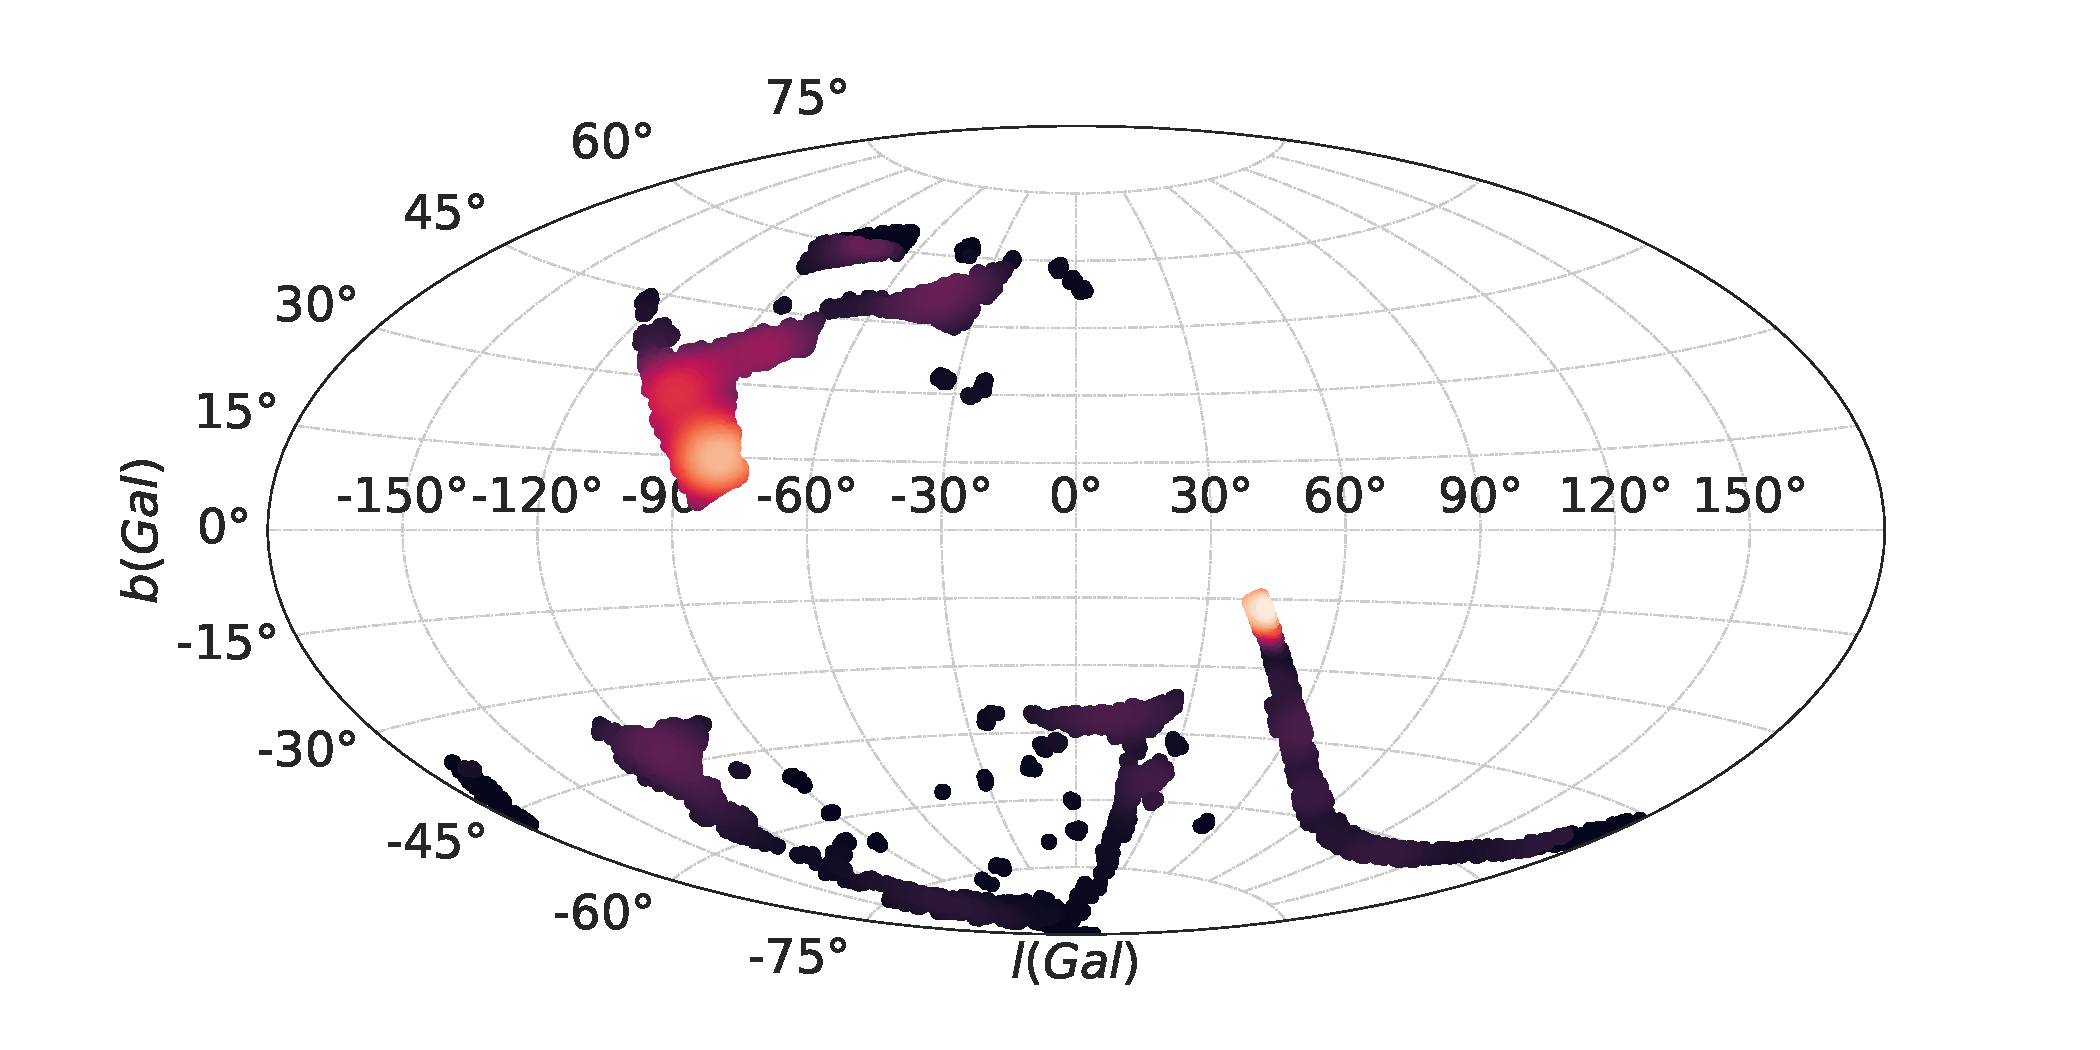
\includegraphics[width=\columnwidth]{Figs/halpha-emitters-galactic-aitoff.pdf}
    \caption{Emission lines selected...}
    \label{fig:distribution}
\end{figure}

% Example figure
%% \begin{figure}
%% 	% To include a figure from a file named example.*
%% 	% Allowable file formats are eps or ps if compiling using latex
%% 	% or pdf, png, jpg if compiling using pdflatex
%% 	\includegraphics[width=\columnwidth]{example}
%%     \caption{This is an example figure. Captions appear below each figure.
%% 	Give enough detail for the reader to understand what they're looking at,
%% 	but leave detailed discussion to the main body of the text.}
%%     \label{fig:example_figure}
%% \end{figure}

% Example table
%% \begin{table}
%% 	\centering
%% 	\caption{This is an example table. Captions appear above each table.
%% 	Remember to define the quantities, symbols and units used.}
%% 	\label{tab:example_table}
%% 	\begin{tabular}{lccr} % four columns, alignment for each
%% 		\hline
%% 		A & B & C & D\\
%% 		\hline
%% 		1 & 2 & 3 & 4\\
%% 		2 & 4 & 6 & 8\\
%% 		3 & 5 & 7 & 9\\
%% 		\hline
%% 	\end{tabular}
%% \end{table}


\section{Conclusions}


\section*{Acknowledgements}


%%%%%%%%%%%%%%%%%%%%%%%%%%%%%%%%%%%%%%%%%%%%%%%%%%
\section*{Data Availability}





%%%%%%%%%%%%%%%%%%%% REFERENCES %%%%%%%%%%%%%%%%%%

% The best way to enter references is to use BibTeX:

\bibliographystyle{mnras}
\bibliography{example} % if your bibtex file is called example.bib


% Alternatively you could enter them by hand, like this:
% This method is tedious and prone to error if you have lots of references
%\begin{thebibliography}{99}
%\bibitem[\protect\citeauthoryear{Author}{2012}]{Author2012}
%Author A.~N., 2013, Journal of Improbable Astronomy, 1, 1
%\bibitem[\protect\citeauthoryear{Others}{2013}]{Others2013}
%Others S., 2012, Journal of Interesting Stuff, 17, 198
%\end{thebibliography}

%%%%%%%%%%%%%%%%%%%%%%%%%%%%%%%%%%%%%%%%%%%%%%%%%%

%%%%%%%%%%%%%%%%% APPENDICES %%%%%%%%%%%%%%%%%%%%%

\appendix

\section{Some extra material}


%%%%%%%%%%%%%%%%%%%%%%%%%%%%%%%%%%%%%%%%%%%%%%%%%%


% Don't change these lines
\bsp	% typesetting comment
\label{lastpage}
\end{document}

% End of mnras_template.tex
